%\appendix
\newpage
\section*{Annexe I : Synthèse FRF}

\begin{equation}
  \frac{1}{Y_{total}} = \frac{1}{Y_{body}} + \frac{1}{Y_{string}}
  \label{eq:eq_frf_1}
\end{equation}

\begin{equation}
  \frac{\delta_{bridge}}{F_{excitation}} = \frac{\delta_{excitation}}{F_{bridge}} = \frac{Y_{total}H}{j\omega}
  \label{eq:eq_frf_2}
\end{equation}

\begin{equation}
	\omega_n = n\omega_0\left(1+\frac{B}{2T}(\frac{n\pi}{L})^2\right)
 \label{eq:eq_frf_3}
\end{equation}


\begin{equation}
 Z(\omega) = -\frac{iT}{L} \left[ \frac{1}{\omega} + \sum_{j=1}^{\infty} \left\lbrace \frac{1}{\omega - \omega_j (1+ i\eta_j/2)} + \frac{1}{\omega + \omega_j (1+ i\eta_j/2)} \right\rbrace  \right]
  \label{eq:eq_frf_4}
\end{equation}

\begin{equation}
H(\omega) = \frac{y}{w} = \frac{c}{L} sin(\omega x/c )\sum_n (-1)^n \frac{1}{\omega - \omega_n(1 + i\eta_n)}
  \label{eq:eq_frf_5}
\end{equation}

\section*{Annexe II : Implémentation}

Le code du projet est disponible publiquement sur GitHub à l'adresse :
\url{https://github.com/PAM-ATIAM-JLLC-BD-2015-2016/octo-couscous-omega}

Des exemples de sons de synthèse au format WAV sont disponibles dans ce même dépôt Git,
dans le sous-dossier :
\url{https://github.com/PAM-ATIAM-JLLC-BD-2015-2016/octo-couscous-omega/tree/master/sounds}


\section*{Annexe III : Dispositif de mesures}

\begin{figure}[hpbt]
\centering
   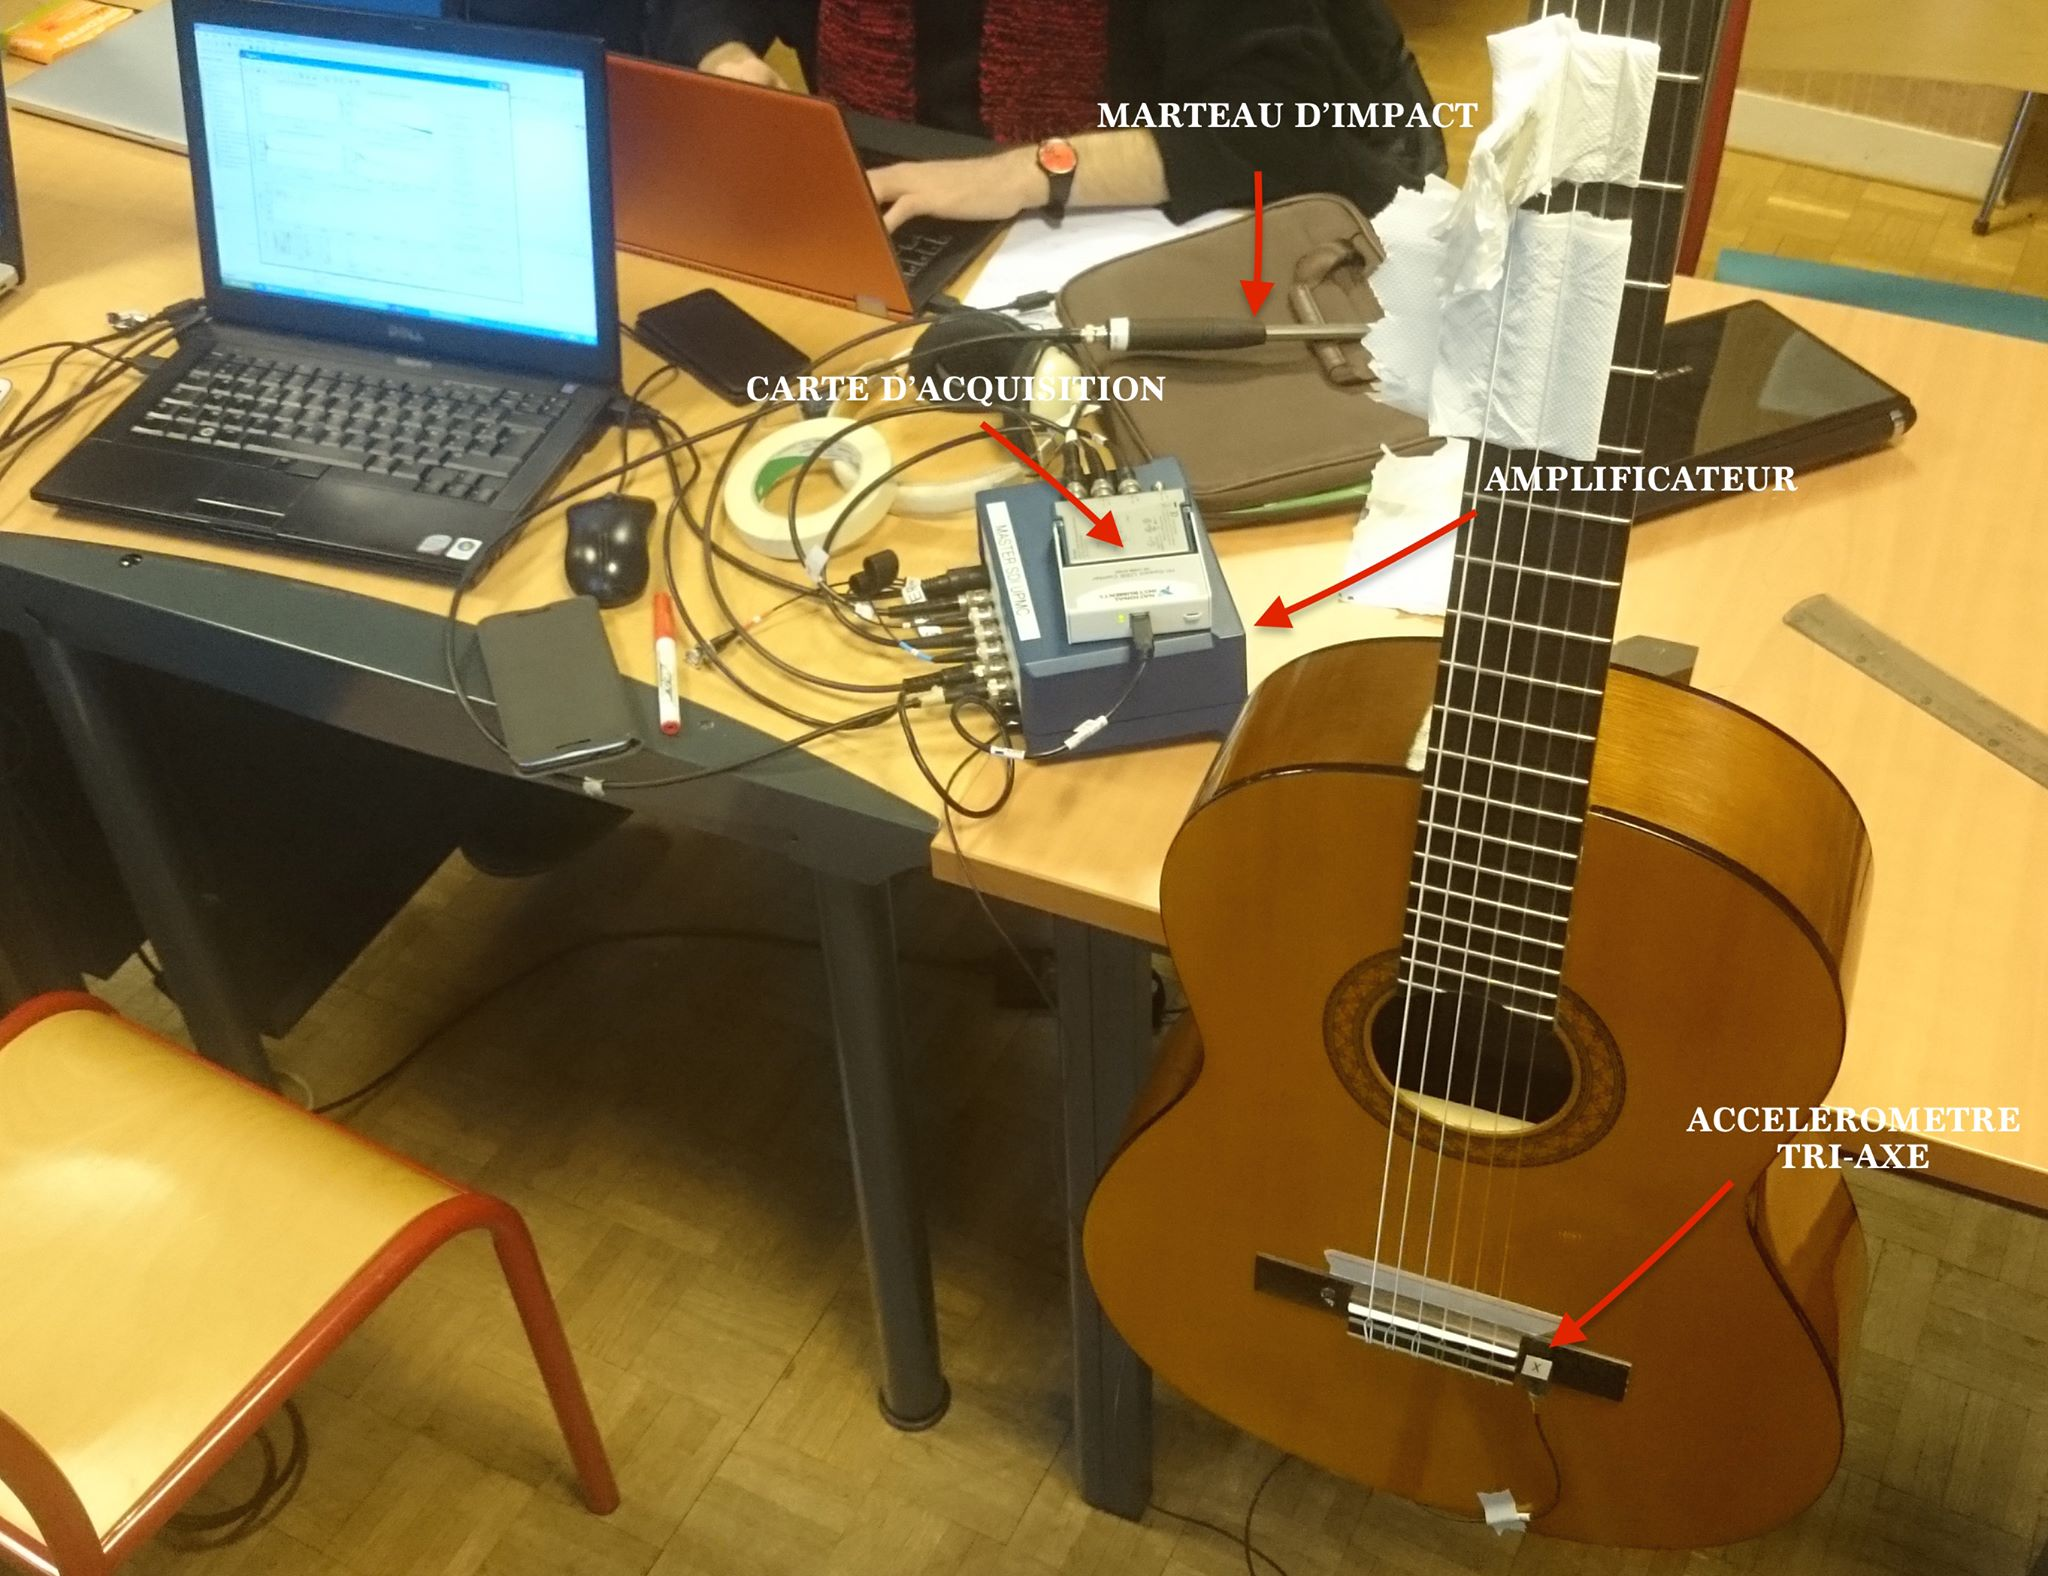
\includegraphics[scale=0.15]{figures/dispo.jpg}
\caption{Dispositif utilisé lors des mesures effectuées au LAM\label{fig:disp}}
\end{figure}